\documentclass{article}%
\usepackage[T1]{fontenc}%
\usepackage[utf8]{inputenc}%
\usepackage{lmodern}%
\usepackage{textcomp}%
\usepackage{lastpage}%
\usepackage{geometry}%
\geometry{margin=0.5in}%
\usepackage{ragged2e}%
\usepackage{graphicx}%
%
\title{{[}WMedSeaExample{]}: SPASSO Images Analysis}%
\author{John Doe}%
\date{\today}%
%
\begin{document}%
\normalsize%
\maketitle%
\begin{center}%
**********************************************%
\textbf{\newline%
Executive Summary}%
\newline%
\newline%
 Type here your executive summary\newline%
%
**********************************************%
\end{center}%
\section{Ongoing operations and upcoming stations}%
\label{sec:Ongoingoperationsandupcomingstations}%
Type here.

%
\section{Daily figures analysis}%
\label{sec:Dailyfiguresanalysis}%
\subsection{Altimetry, derived currents}%
\label{subsec:Altimetry,derivedcurrents}%
Type here.%


\begin{figure}[h!]%
\centering%
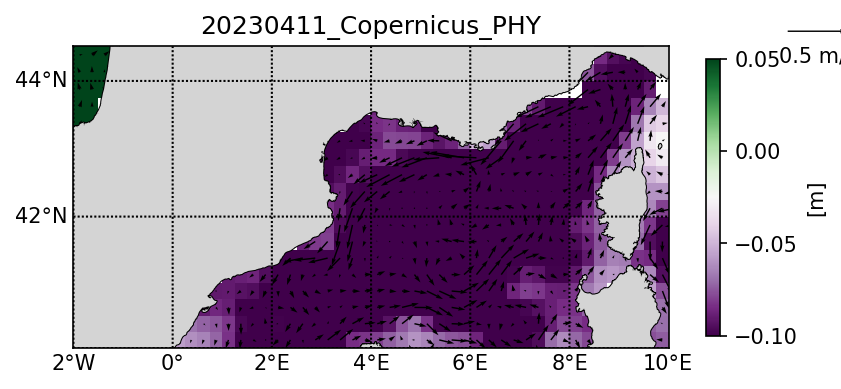
\includegraphics[width=300px]{/Users/lrousselet/LOUISE/SPASSO/GitHubRELEASE/SPASSO/Cruises/WMedSeaExample/Wrk/20230411_Copernicus_PHY_0.png}%
\end{figure}

%
\clearpage

%
\subsection{SST analysis}%
\label{subsec:SSTanalysis}%
Type here.%


\begin{figure}[h!]%
\centering%
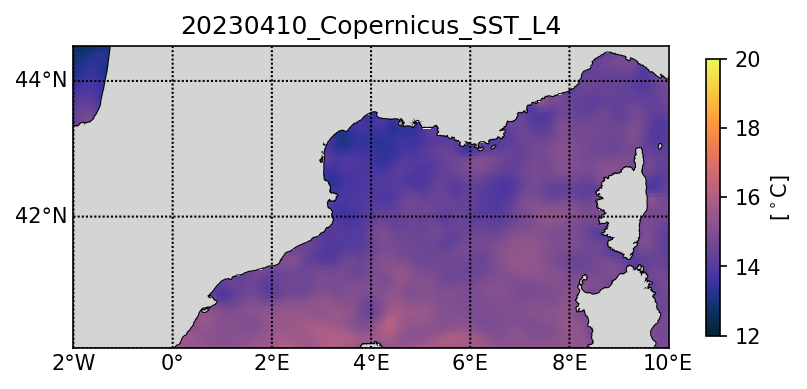
\includegraphics[width=300px]{/Users/lrousselet/LOUISE/SPASSO/GitHubRELEASE/SPASSO/Cruises/WMedSeaExample/Wrk/20230410_Copernicus_SST_L4_0.png}%
\end{figure}

%
\clearpage

%
\subsection{Chlorophyll analysis}%
\label{subsec:Chlorophyllanalysis}%
Type here.%


\begin{figure}[h!]%
\centering%
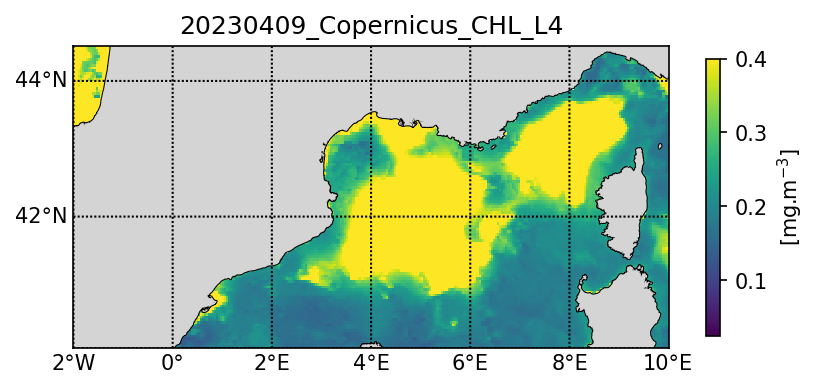
\includegraphics[width=300px]{/Users/lrousselet/LOUISE/SPASSO/GitHubRELEASE/SPASSO/Cruises/WMedSeaExample/Wrk/20230409_Copernicus_CHL_L4_0.png}%
\end{figure}

%
\clearpage

%
\subsection{Eulerian/Lagrangian analysis}%
\label{subsec:Eulerian/Lagrangiananalysis}%
Eulerian diagnostics computed with Copernicus\_PHY velocities:\newline%
 KE: kinetic energy \newline%
 OW: Okubo{-}Weiss parameter\newline%
\newline%
%
 Lagrangian diagnostics computed by seeding Lagrangian particles every 0.02deg and advected for 30 days backward in time with Copernicus\_PHY velocities:\newline%
FTLE: finite time Lyapunov exponents (convergent fronts detection)\newline%
LLADV: longitude and latitude advection\newline%
Retention parameter (based on computing the okubo Weiss parameter along a particle trajectory): Detect trapping structures (colorbar = days water parcels have a positive vorticity)\newline%
Timefrombathy: Water age since last contact with isobath XXm (precised in figure title)\newline%
\newline%
More details available at: https://www.swot{-}adac.org/resources/swot{-}adac{-}products{-}access/ \newline%
\newline%
%


\begin{figure}[h!]%
\centering%
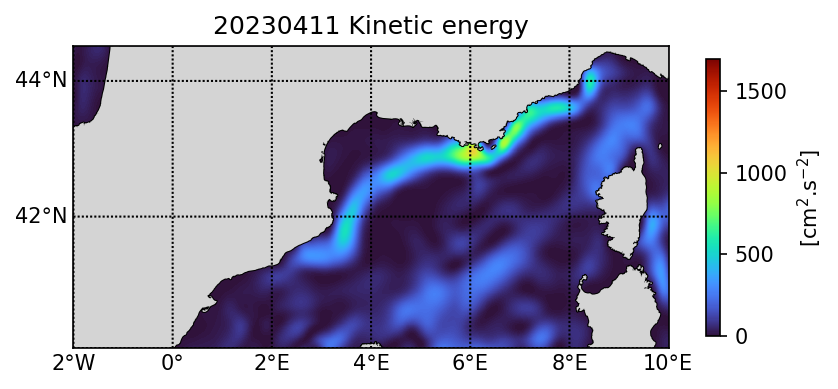
\includegraphics[width=300px]{/Users/lrousselet/LOUISE/SPASSO/GitHubRELEASE/SPASSO/Cruises/WMedSeaExample/Wrk/20230411_KE_Copernicus_PHY_0.png}%
\end{figure}

%


\begin{figure}[h!]%
\centering%
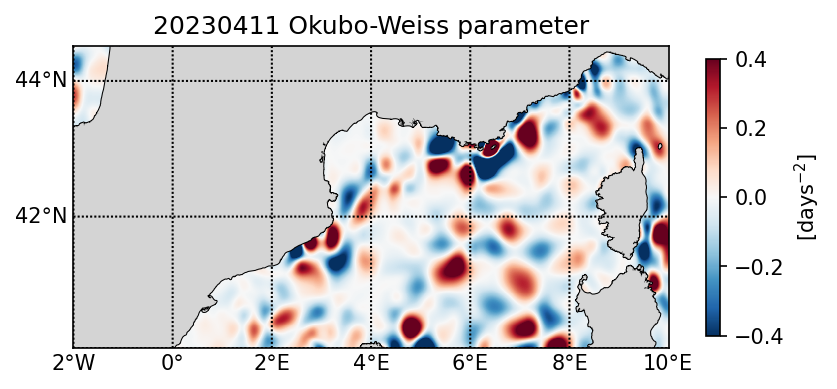
\includegraphics[width=300px]{/Users/lrousselet/LOUISE/SPASSO/GitHubRELEASE/SPASSO/Cruises/WMedSeaExample/Wrk/20230411_OW_Copernicus_PHY_0.png}%
\end{figure}

%


\begin{figure}[h!]%
\centering%
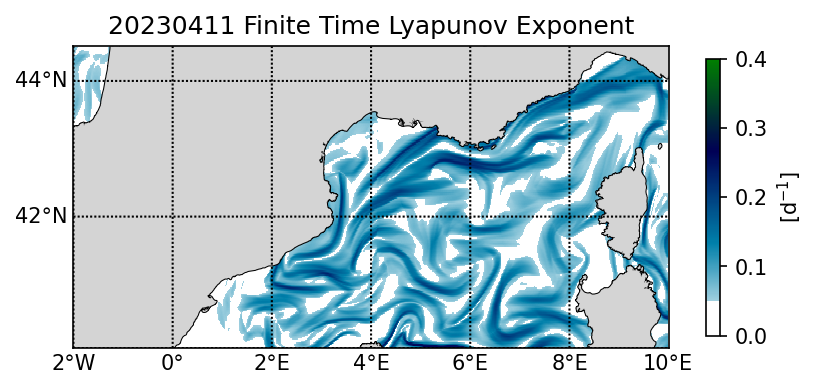
\includegraphics[width=300px]{/Users/lrousselet/LOUISE/SPASSO/GitHubRELEASE/SPASSO/Cruises/WMedSeaExample/Wrk/20230411_FTLE_Copernicus_PHY_0.png}%
\end{figure}

%
\clearpage

%
\subsection{Other analysis}%
\label{subsec:Otheranalysis}%
Type here.

%
\begin{center}%
\textbf{Acknowledgments}%
\end{center}%
Type here.%
\end{document}